%%%%%%%%%%%%%%%%%%%%%%%%%%%%%%%%%%%%%%%%%%%%%%%%%%%%%%%%%%%%%%%%%%%%%%%%%%%%%
%% Original default rstudio/pandoc latex file
%% upated by @jhollist 09/15/2014
%% inspired by @cboetting https://github.com/cboettig/template and
%% @rmflight blog posts:
%% http://rmflight.github.io/posts/2014/07/analyses_as_packages.html 
%% http://rmflight.github.io/posts/2014/07/vignetteAnalysis.html).  
%%%%%%%%%%%%%%%%%%%%%%%%%%%%%%%%%%%%%%%%%%%%%%%%%%%%%%%%%%%%%%%%%%%%%%%%%%%%%

\documentclass[11pt,]{article}
\usepackage[T1]{fontenc}
\usepackage{lmodern}
\usepackage{amssymb,amsmath}
\usepackage{ifxetex,ifluatex}
\usepackage{fixltx2e} % provides \textsubscript
% use upquote if available, for straight quotes in verbatim environments
\IfFileExists{upquote.sty}{\usepackage{upquote}}{}
\ifnum 0\ifxetex 1\fi\ifluatex 1\fi=0 % if pdftex
  \usepackage[utf8]{inputenc}
\else % if luatex or xelatex
  \ifxetex
    \usepackage{mathspec}
    \usepackage{xltxtra,xunicode}
  \else
    \usepackage{fontspec}
  \fi
  \defaultfontfeatures{Mapping=tex-text,Scale=MatchLowercase}
  \newcommand{\euro}{€}
\fi
% use microtype if available
\IfFileExists{microtype.sty}{\usepackage{microtype}}{}
\usepackage{longtable,booktabs}
\usepackage{graphicx}
% Redefine \includegraphics so that, unless explicit options are
% given, the image width will not exceed the width of the page.
% Images get their normal width if they fit onto the page, but
% are scaled down if they would overflow the margins.
\makeatletter
\def\ScaleIfNeeded{%
  \ifdim\Gin@nat@width>\linewidth
    \linewidth
  \else
    \Gin@nat@width
  \fi
}
\makeatother
\let\Oldincludegraphics\includegraphics
{%
 \catcode`\@=11\relax%
 \gdef\includegraphics{\@ifnextchar[{\Oldincludegraphics}{\Oldincludegraphics[width=\ScaleIfNeeded]}}%
}%
\ifxetex
  \usepackage[setpagesize=false, % page size defined by xetex
              unicode=false, % unicode breaks when used with xetex
              xetex]{hyperref}
\else
  \usepackage[unicode=true]{hyperref}
\fi
\hypersetup{breaklinks=true,
            bookmarks=true,
            pdfauthor={},
            pdftitle={Associations between Chlorophyll a and Microcystin-LR Health Advisory Concentrations},
            colorlinks=true,
            citecolor=blue,
            urlcolor=blue,
            linkcolor=magenta,
            pdfborder={0 0 0}}
\urlstyle{same}  % don't use monospace font for urls
\setlength{\parindent}{0pt}
\setlength{\parskip}{6pt plus 2pt minus 1pt}
\setlength{\emergencystretch}{3em}  % prevent overfull lines
\setcounter{secnumdepth}{5}

%%%%%%%%%%%%%%%%%%%%%%%%%%%%%%%%%%%%%%%%%%%%%%%%%%%%%%%%
%Changes borrowed from @cboettig, added by @jhollist 
% A modified page layout 
\textwidth 6.75in
\oddsidemargin -0.15in
\evensidemargin -0.15in
\textheight 9in
\topmargin -0.5in
\usepackage{lineno} % add 
%%%%%%%%%%%%%%%%%%%%%%%%%%%%%%%%%%%%%%%%%%%%%%%%%%%%%%%%

%%%%%%%%%%%%%%%%%%%%%%%%%%%%%%%%%%%%%%%%%%%%%%%%%%%%%%%%
%%Packages and layout changes by @jhollist 09/15/2014
\usepackage{ragged2e}
\usepackage[font=normalsize]{caption}
  \usepackage[doublespacing]{setspace}
\usepackage{parskip}
\usepackage{fancyhdr}
\pagestyle{fancy}
\fancyhf{}
\renewcommand{\headrulewidth}{0pt}
\rfoot{\today}
\lfoot{\thepage}
%%Changed default abstract width and added lines
\renewenvironment{abstract}{
  \hfill\begin{minipage}{1\textwidth}
  \rule{\textwidth}{1pt}\vspace{5pt}
  \normalsize
  \begin{justify}
  \bfseries\abstractname\vspace{5pt}
  \end{justify}}
  {\par\noindent\rule{\textwidth}{1pt}\end{minipage}
}
%%%%%%%%%%%%%%%%%%%%%%%%%%%%%%%%%%%%%%%%%%%%%%%%%%%%%%%%

\title{Associations between Chlorophyll \emph{a} and Microcystin-LR Health
Advisory Concentrations}
\author{
Jeffrey W. Hollister
Betty J. Kreakie
Dorothy Q. Kellog
}
\date{}

\begin{document}
%%Edited by @jhollist 09/15/2014
%%Adds title from YAML
\begin{singlespace}
\begin{center}
\huge Associations between Chlorophyll \emph{a} and Microcystin-LR Health
Advisory Concentrations
\end{center}
%%Adds Author, correspond email asterisk, and affilnum from YAML
\begin{center}
\large
Jeffrey W. Hollister \textsuperscript{*} \textsuperscript{1} 
Betty J. Kreakie \textsuperscript{1} 
Dorothy Q. Kellog \textsuperscript{2} 
\end{center}
%%Adds affiliations from YAML
\begin{justify}
\footnotesize \emph{ 
\\*
\textsuperscript{1}US Environmental Protection Agency, Office of Research and Development,
National Health and Environmental Effects Research Laboratory, Atlantic
Ecology Division, 27 Tarzwell Drive Narragansett, RI, 02882, USA\\*
\\*
\textsuperscript{2}University of Rhode Island, Department of Natural Resrouces Science,
Kingston, RI, 02882, USA\\*
}
%%Adds corresponding author email(s) from YAML
\newcounter{num}
\setcounter{num}{1}
\\[0.1cm]
\footnotesize \emph{ 
\ifnum\value{num}=1%
\textsuperscript{*} corresponding author:
\fi
\href{mailto:hollister.jeff@epa.gov}{\nolinkurl{hollister.jeff@epa.gov}}
\stepcounter{num}
}
\end{justify}
%%Adds date from YAML
\normalsize

\end{singlespace}


\singlespace

\vspace{2mm}

\hrule

\vspace{3mm}

\hrule

\doublespace

\section{Introduction}\label{introduction}

\section{Methods}\label{methods}

\begin{longtable}[c]{@{}lll@{}}
\toprule
\begin{minipage}[b]{0.27\columnwidth}\raggedright\strut
Source
\strut\end{minipage} &
\begin{minipage}[b]{0.16\columnwidth}\raggedright\strut
Type
\strut\end{minipage} &
\begin{minipage}[b]{0.19\columnwidth}\raggedright\strut
Concentration
\strut\end{minipage}\tabularnewline
\midrule
\endhead
\begin{minipage}[t]{0.27\columnwidth}\raggedright\strut
WHO, OH, OR
\strut\end{minipage} &
\begin{minipage}[t]{0.16\columnwidth}\raggedright\strut
Drinking
\strut\end{minipage} &
\begin{minipage}[t]{0.19\columnwidth}\raggedright\strut
1 ug/l
\strut\end{minipage}\tabularnewline
\begin{minipage}[t]{0.27\columnwidth}\raggedright\strut
MN
\strut\end{minipage} &
\begin{minipage}[t]{0.16\columnwidth}\raggedright\strut
Drinking
\strut\end{minipage} &
\begin{minipage}[t]{0.19\columnwidth}\raggedright\strut
0.04 ug/l
\strut\end{minipage}\tabularnewline
\begin{minipage}[t]{0.27\columnwidth}\raggedright\strut
U.S. EPA
\strut\end{minipage} &
\begin{minipage}[t]{0.16\columnwidth}\raggedright\strut
Drinking
\strut\end{minipage} &
\begin{minipage}[t]{0.19\columnwidth}\raggedright\strut
0.3 ug/l
\strut\end{minipage}\tabularnewline
\begin{minipage}[t]{0.27\columnwidth}\raggedright\strut
U.S. EPA
\strut\end{minipage} &
\begin{minipage}[t]{0.16\columnwidth}\raggedright\strut
Drinking
\strut\end{minipage} &
\begin{minipage}[t]{0.19\columnwidth}\raggedright\strut
1.6 ug/l
\strut\end{minipage}\tabularnewline
\begin{minipage}[t]{0.27\columnwidth}\raggedright\strut
WHO, IN
\strut\end{minipage} &
\begin{minipage}[t]{0.16\columnwidth}\raggedright\strut
Recreational
\strut\end{minipage} &
\begin{minipage}[t]{0.19\columnwidth}\raggedright\strut
2-4 ug/l
\strut\end{minipage}\tabularnewline
\begin{minipage}[t]{0.27\columnwidth}\raggedright\strut
WHO, IN, KS
\strut\end{minipage} &
\begin{minipage}[t]{0.16\columnwidth}\raggedright\strut
Recreational
\strut\end{minipage} &
\begin{minipage}[t]{0.19\columnwidth}\raggedright\strut
10-20 ug/l
\strut\end{minipage}\tabularnewline
\begin{minipage}[t]{0.27\columnwidth}\raggedright\strut
WHO, IN, IA, KS, NE, OH
\strut\end{minipage} &
\begin{minipage}[t]{0.16\columnwidth}\raggedright\strut
Recreational
\strut\end{minipage} &
\begin{minipage}[t]{0.19\columnwidth}\raggedright\strut
20-2000 ug/l
\strut\end{minipage}\tabularnewline
\begin{minipage}[t]{0.27\columnwidth}\raggedright\strut
WHO
\strut\end{minipage} &
\begin{minipage}[t]{0.16\columnwidth}\raggedright\strut
Recreational
\strut\end{minipage} &
\begin{minipage}[t]{0.19\columnwidth}\raggedright\strut
\textgreater{}2000 ug/l
\strut\end{minipage}\tabularnewline
\begin{minipage}[t]{0.27\columnwidth}\raggedright\strut
CA
\strut\end{minipage} &
\begin{minipage}[t]{0.16\columnwidth}\raggedright\strut
Recreational
\strut\end{minipage} &
\begin{minipage}[t]{0.19\columnwidth}\raggedright\strut
0.8 ug/l
\strut\end{minipage}\tabularnewline
\begin{minipage}[t]{0.27\columnwidth}\raggedright\strut
IL, OR
\strut\end{minipage} &
\begin{minipage}[t]{0.16\columnwidth}\raggedright\strut
Recreational
\strut\end{minipage} &
\begin{minipage}[t]{0.19\columnwidth}\raggedright\strut
10 ug/l
\strut\end{minipage}\tabularnewline
\begin{minipage}[t]{0.27\columnwidth}\raggedright\strut
MA, RI
\strut\end{minipage} &
\begin{minipage}[t]{0.16\columnwidth}\raggedright\strut
Recreational
\strut\end{minipage} &
\begin{minipage}[t]{0.19\columnwidth}\raggedright\strut
14 ug/l
\strut\end{minipage}\tabularnewline
\begin{minipage}[t]{0.27\columnwidth}\raggedright\strut
OH, VT, VA, WA
\strut\end{minipage} &
\begin{minipage}[t]{0.16\columnwidth}\raggedright\strut
Recreational
\strut\end{minipage} &
\begin{minipage}[t]{0.19\columnwidth}\raggedright\strut
6 ug/l
\strut\end{minipage}\tabularnewline
\bottomrule
\end{longtable}

Based on the range of microcystin concentrations used in various policy
settings, we evaulated associated chlorohpyll \emph{a} concentrations
for an effect at 0.04, 0.3, 0.8, 1, 1.6, 4, 6, 10, 14, and 20 ug/l.

\subsection{Data and Study Area}\label{data-and-study-area}

\section{Results}\label{results}

\section{Discussion}\label{discussion}

\section{Figures}\label{figures}

\begin{figure}[htbp]
\centering
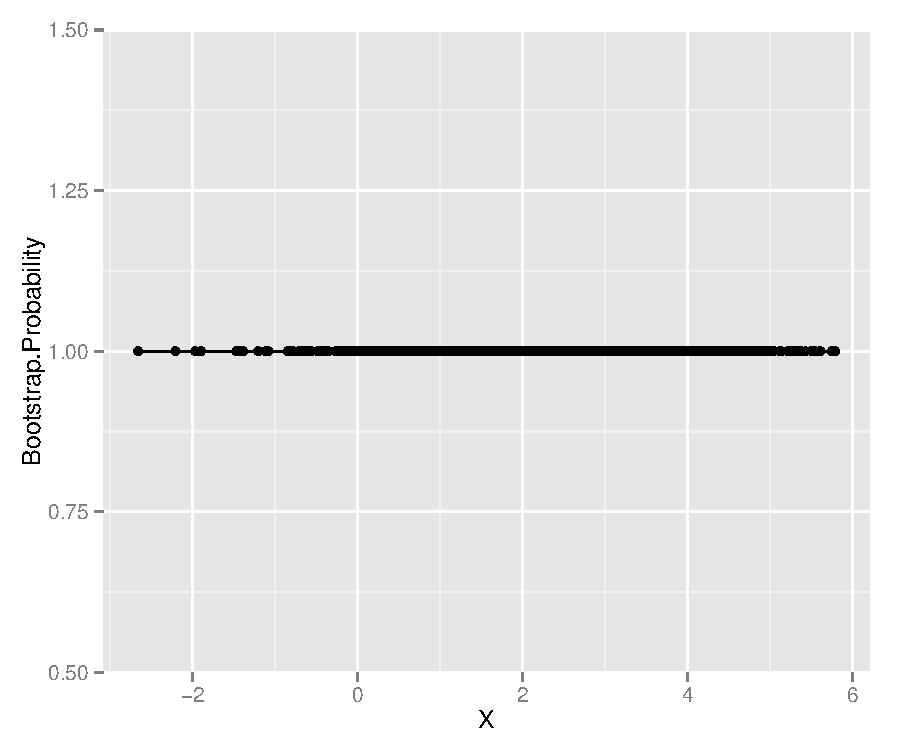
\includegraphics{manuscript_files/figure-latex/mn_cp_plot-1.pdf}
\caption{}
\end{figure}

\newpage

\begin{figure}[htbp]
\centering
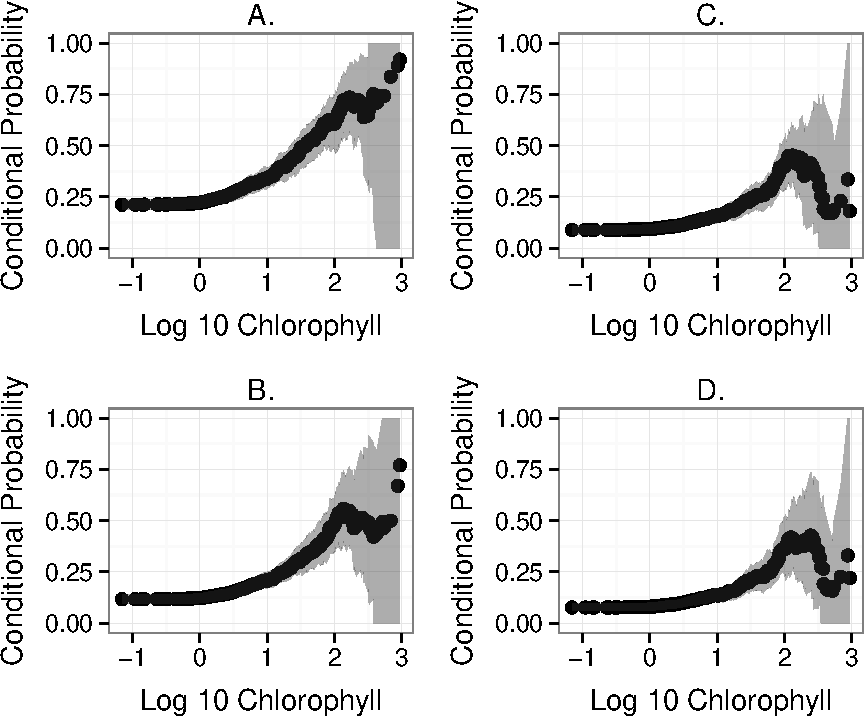
\includegraphics{manuscript_files/figure-latex/epa_child_cp_plot-1.pdf}
\caption{}
\end{figure}

\begin{figure}[htbp]
\centering
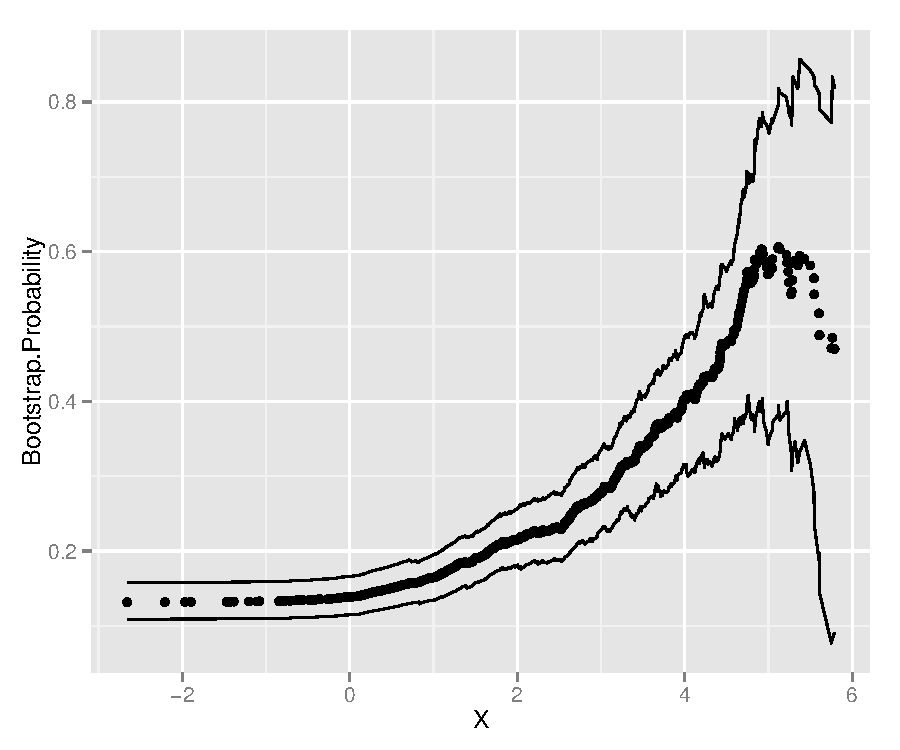
\includegraphics{manuscript_files/figure-latex/ca_cp_plot-1.pdf}
\caption{}
\end{figure}

\newpage

\begin{figure}[htbp]
\centering
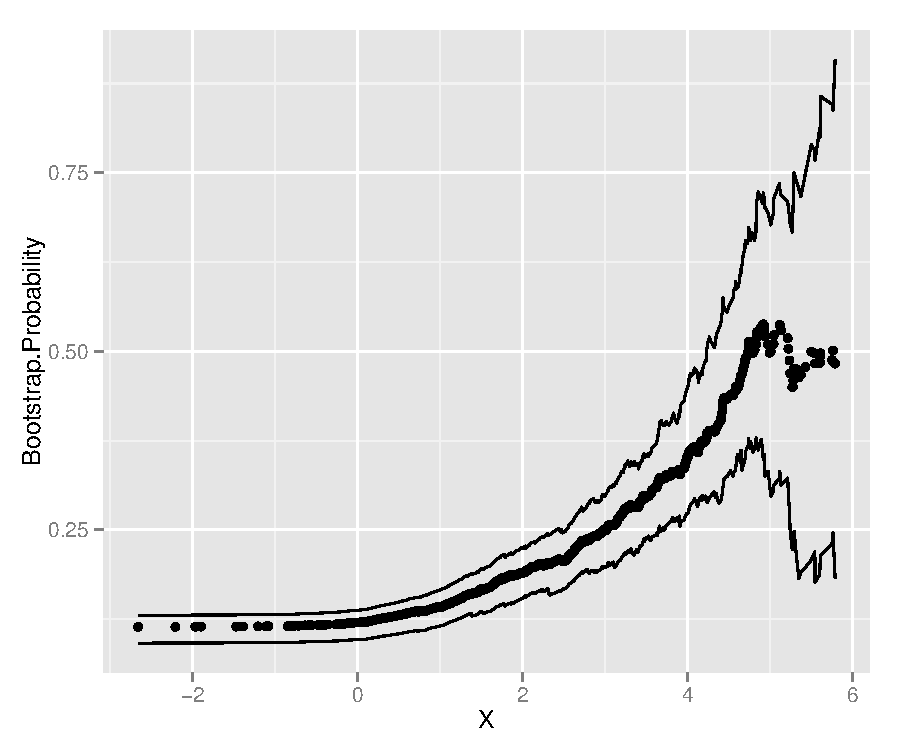
\includegraphics{manuscript_files/figure-latex/who_drink_cp_plot-1.pdf}
\caption{}
\end{figure}

\newpage

\begin{figure}[htbp]
\centering
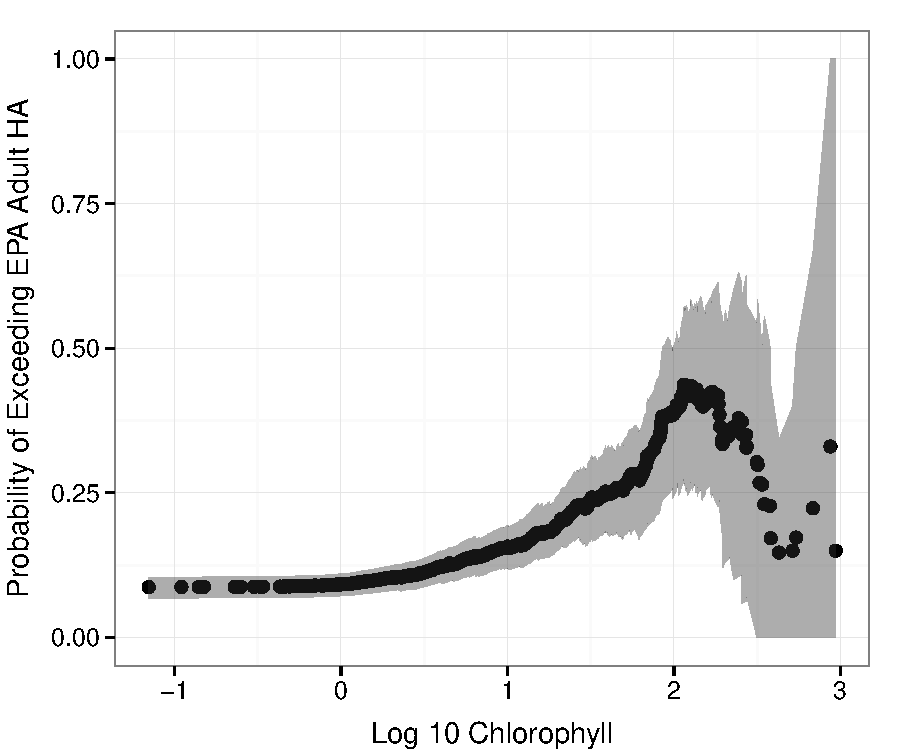
\includegraphics{manuscript_files/figure-latex/epa_adult_cp -1.pdf}
\caption{}
\end{figure}

\newpage

\begin{figure}[htbp]
\centering
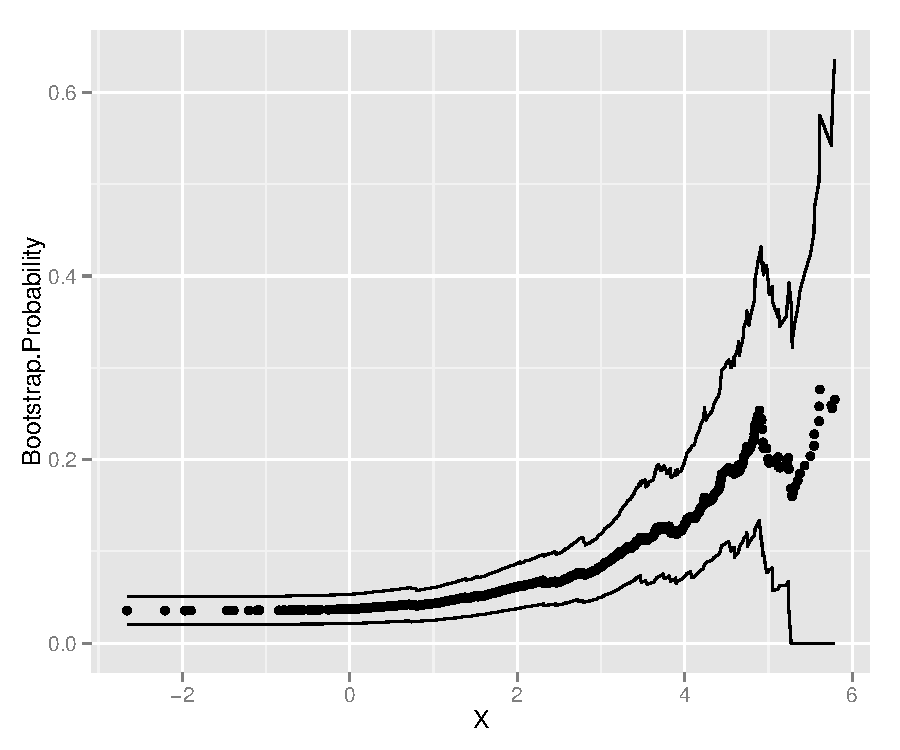
\includegraphics{manuscript_files/figure-latex/who_rec_low_cp-1.pdf}
\caption{}
\end{figure}

\newpage

\begin{figure}[htbp]
\centering
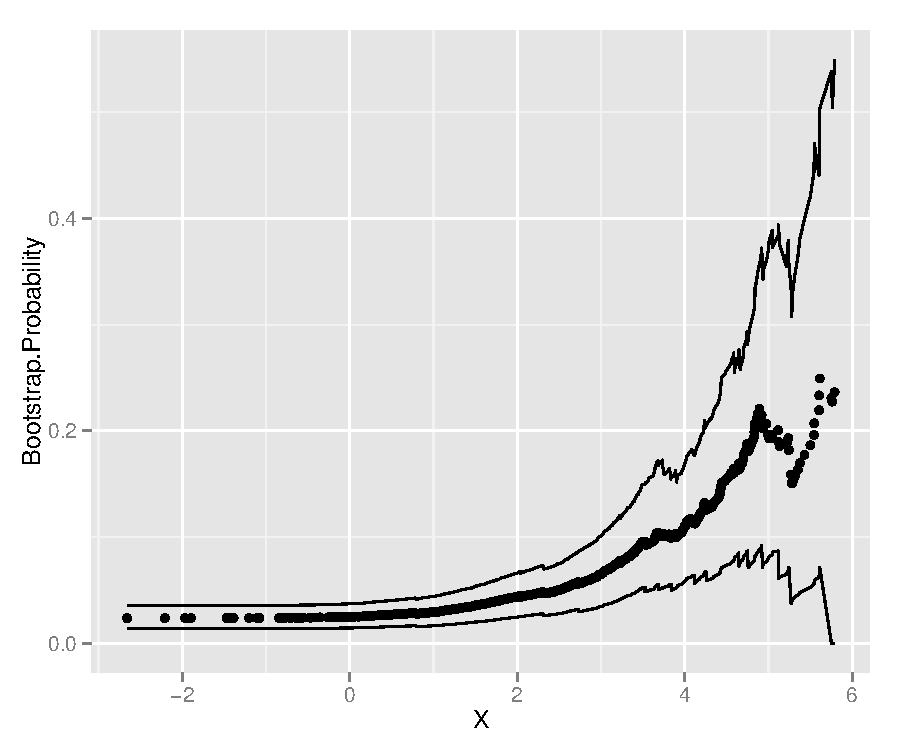
\includegraphics{manuscript_files/figure-latex/mult_state_rec_cp-1.pdf}
\caption{}
\end{figure}

\newpage

\begin{figure}[htbp]
\centering
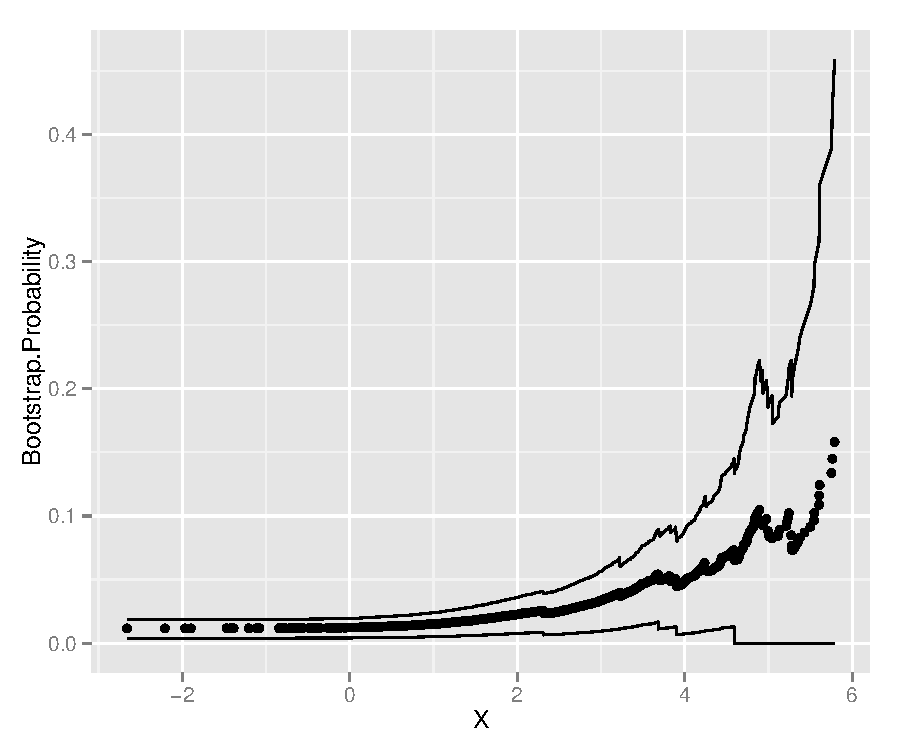
\includegraphics{manuscript_files/figure-latex/il_org_cp-1.pdf}
\caption{}
\end{figure}

\newpage

\begin{figure}[htbp]
\centering
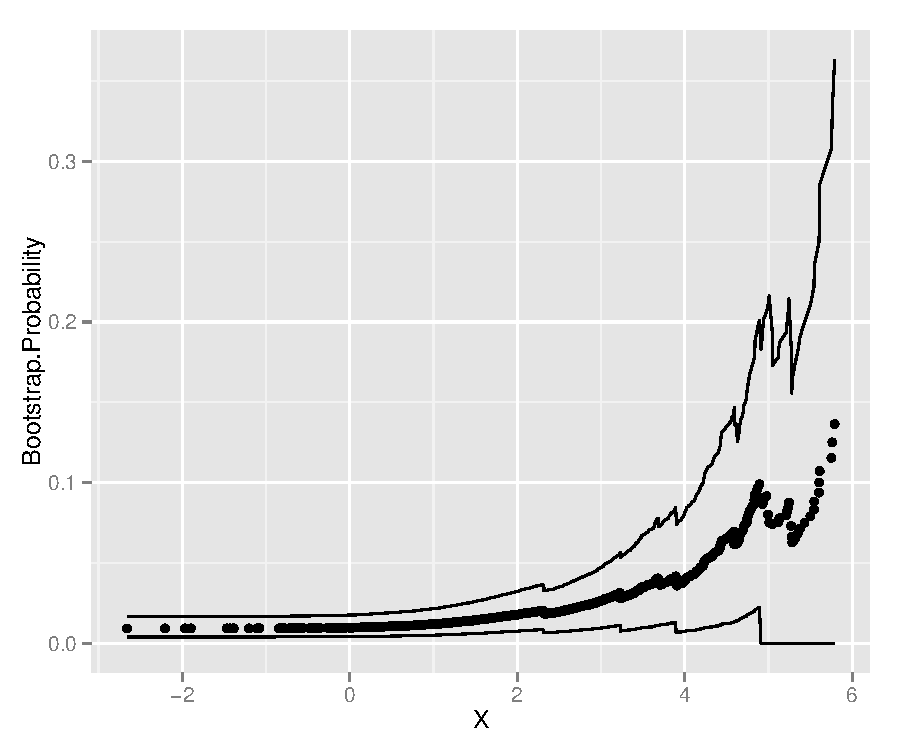
\includegraphics{manuscript_files/figure-latex/ma_ri_cp-1.pdf}
\caption{}
\end{figure}

\newpage

\begin{figure}[htbp]
\centering
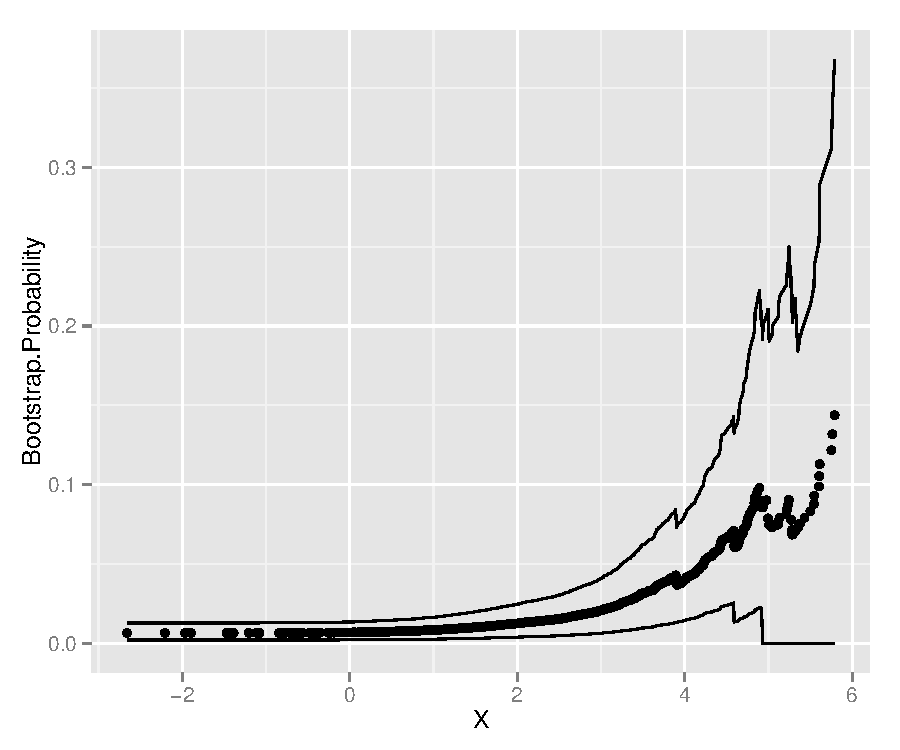
\includegraphics{manuscript_files/figure-latex/who_rec_med_cp-1.pdf}
\caption{}
\end{figure}

\newpage

\section*{References}\label{references}
\addcontentsline{toc}{section}{References}

\end{document}